\documentclass[12pt]{article}

% PACKAGES
\usepackage{geometry}                                        % page setup
\usepackage{graphicx}                                        % picture inserting
\usepackage{setspace}                                        % set spacing
\usepackage{indentfirst}                                     % indent the first paragraph of each section
\usepackage{hyperref}                                        % adds hyperlinks between sections and TOC
\usepackage{amsmath}                                         % adds support for math stuff
\usepackage{csvsimple}                                       % csv importing?
\usepackage[T1]{fontenc}                                     % adds extra font encoding
\usepackage{lmodern}                                         % fixes font glitches when updating encoding
\usepackage[nottoc,notlot,notlof]{tocbibind}                 % remove TOC, LOT, and LOF from TOC
\usepackage[style=ieee,sorting=anyt,backend=biber]{biblatex} % bibliography

% DOCUMENT SETTINGS
% PAPER SETTINGS
\geometry{letterpaper,
          left=1in,
          right=1in,
          top=1in,
          bottom=1in}

% IMAGE DIRECTORY
\graphicspath{{images/}}

% OTHER SETTINGS
\renewcommand*\contentsname{Table of Contents} % change table of contents name
\renewcommand{\thefigure}{\Roman{figure}}      % make figures have roman numerals
\addbibresource{refs.bib}                      % set the references file

% TITLE DEFINITIONS
\title{Project Lab 3\\\large Interim Report}
\author{Dirk Thieme\\R11636727\\Texas Tech University}
\date{\today}

% MAIN DOCUMENT
\begin{document}
\maketitle % title
\pagenumbering{gobble} % no pg number on title
\newpage
\pagenumbering{arabic} % bring back for everything else
\spacing{2}            % set spacing

% ABSTRACT
\begin{abstract}
    This paper aims to describe the current progress of the LifeMTR body vitals monitoring station. The LifeMTR is a body temperature, blood-oxygen, and heart rate monitoring device which can work independently or in tandem with a live database which can store the recorded data for graphing and future use. The project is currently about half finished, with two printed circuit boards, a mostly working website, and microcontroller code which is almost complete. The project is being developed by Dirk Thieme, Ethan Elliot, and Thompson Nguyen.
\end{abstract}

\newpage
\tableofcontents

\newpage
\listoffigures

\newpage
\section{Introduction}
    The LifeMTR project description is to create a pulse, temperature, and blood-oxygen monitoring system which can also be accessed remotely. While a simple finger mounted USB pulse-oximeter could work just as well, a lot of time and effort has been put in to custom make as much as possible for a working version to truly make it unique.
    
    In order to collect the info from a person, a chest mounted device will be used to allow the user to remain mobile while collection occurs, thus allowing the LifeMTR to be used during exercise or medical events. This device will be mounted using an elastic band that goes under the arms and around the sternum. The main section of device is being 3D modeled using Fusion 360, and after it will be 3D printed and tweaked until satisfied. This part of the project is being saved for later on in the timeline, as making edits to the enclosure is much simpler than changing a PCB or screen placement.
    
    The blood-oxygen levels are collected by a MAX30102, which is a pulse-oximeter and heart rate monitor IC that uses red and infrared LEDs to collect the data \cite{max30102}. Body temperature is found using a MAX30205 body temperature IC which records the temperature of skin \cite{max30205}. The brain of the system is an ESP32, which is a simple microcontroller with built in WiFi and Bluetooth communication \cite{esp32}. Printed circuit boards, furthermore called PCBs, were designed to fit in a handmade enclosure with a small battery and a round LCD screen, which can display the information independently. The LCD is powered by a GC9A01A IC, an LCD controller which uses SPI to interface between the microcontroller and the screen \cite{gc9a01a}.
    
    The software mainly consists of the microcontroller side and the website side. The microcontroller code manages the device itself, from things like WiFi connections, sensor readings, and screen updates, while the website side manages the Firebase database and adds a front end for user access. The microcontroller code is written in C++ using the PlatformIO extension on Visual Studio Code, and the website is written in Javascript. As stated earlier, the database is powered by Google's Firebase, which is a backend as a service used for hosting databases and websites \cite{firebase}.

\newpage
\section{Body}
    The LifeMTR project mainly consists of the software and the hardware. The software is made of the ESP32 code, the Firebase code, and the website code. Figure \ref{fc} show the flowchart for how the code loop works. The hardware is made of the motherboard PCB, the daughter-board PCB, and the physical enclosure.
    \begin{figure}[h]
        \centering
        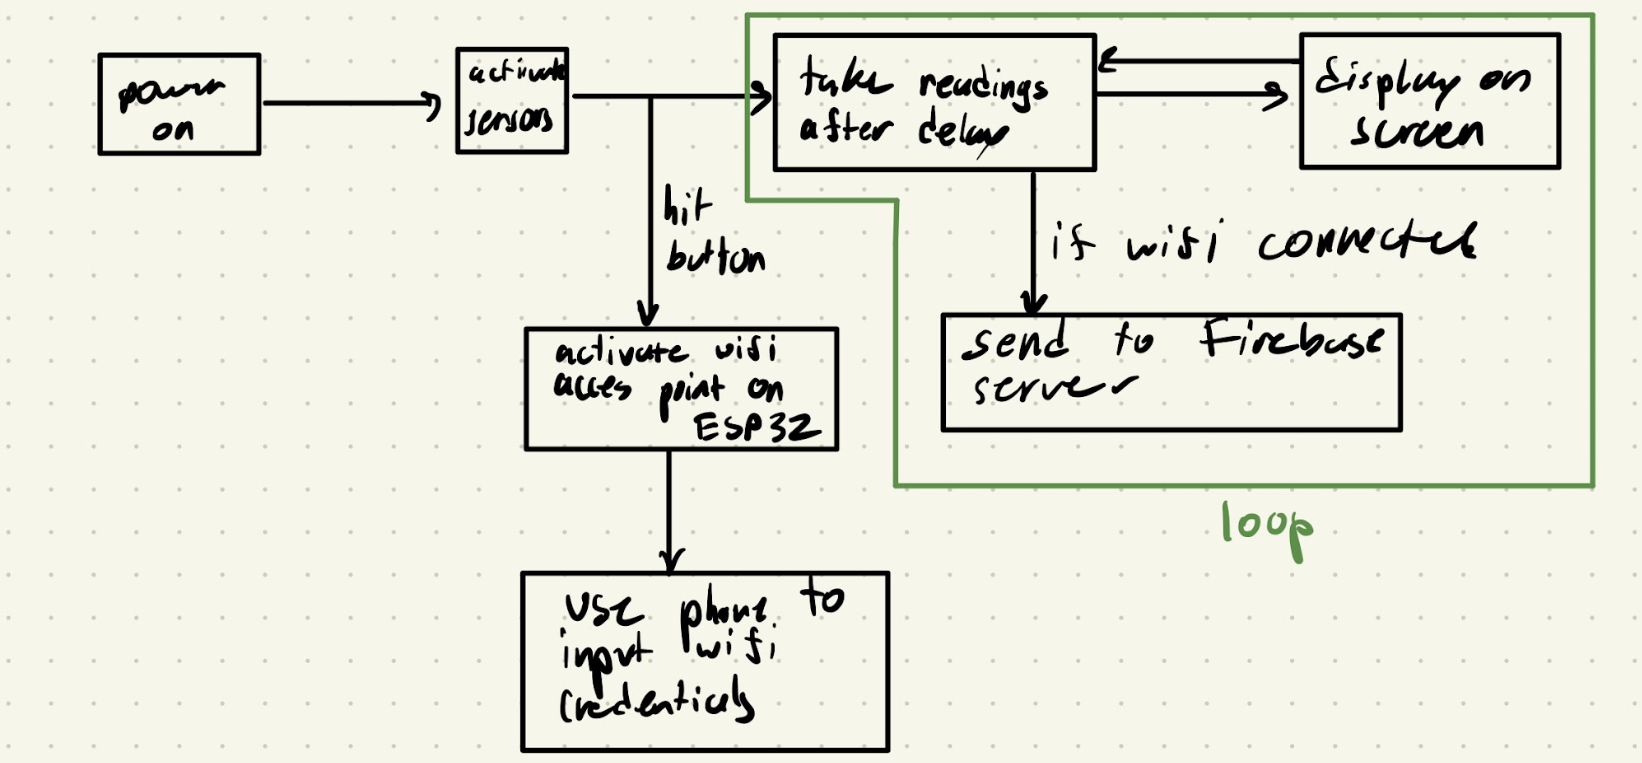
\includegraphics[width=0.75\textwidth]{flowchart}
        \caption{Main Software Flowchart}
        \label{fc}
    \end{figure} 

\subsection{Software}
\subsubsection{Microcontroller}
    As stated earlier, the microcontroller code is written in C++ and is logically broken up into about seven sections. The first section is where all the headers are imported from various libraries. The main libraries used are the TFT\_eSPI library \cite{tft_espi}, the MAX3010x Particle Sensor library \cite{sparkfun_max301x}, the Protocentral MAX30205 Body Temperature sensor library \cite{protocentral_max30205}, the WiFiManager library \cite{wifi_manager}, and the Firebase Realtime Database Client library \cite{firebase_client_lib}. Other libraries are also imported from the ESP32's standard library, such as the I2C library, WiFi library, and the SPI library. This is shown in Figure \ref{uc_lib}.

    \begin{figure}[ht]
        \centering
        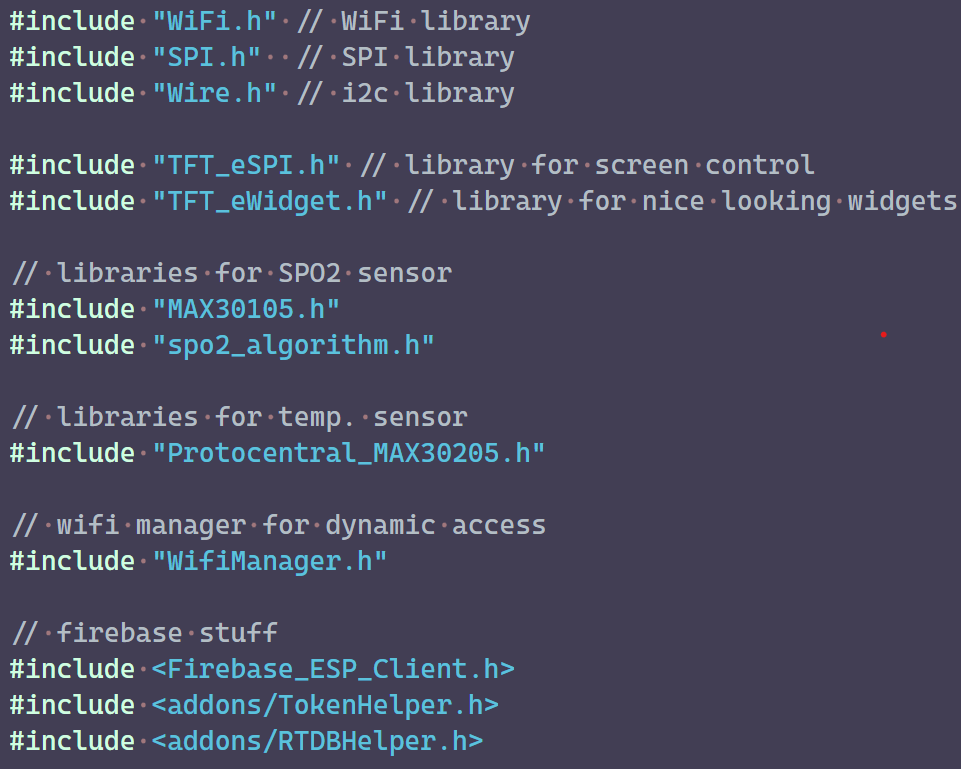
\includegraphics[width=0.75\textwidth]{uc_libs}
        \caption{Microcontroller - Includes}
        \label{uc_lib}
    \end{figure} 

    The code then defines several global variables and define statements which keep track of various things that happen as the code goes along, including flags that keep track of whether WiFi and Firebase are enabled, objects for handling the TFT\_eSPI and the two sensors, arrays for storing pulse oximeter readings, and a few timing variables. A debug flag is also set, which if enabled will allow the ESP32 to communicate back to the device using UART. If the flag is not enabled, the serial connection will never be established, saving power and time \cite{esp32}. Another flag is also used to enable or disable the code which interfaces with the screen, which allow for testing the main important code without having to always have a screen connected. An snippet is shown below in Figure \ref{uc_var} Although the interrupt service routine is small, it is one of the most important functions in the entire program, which is to fire when the button mounted to the motherboard is pressed, it then checks if the WiFi is already enabled, and if not sets a flag for the main loop to startup the WiFi. No real work is done in the ISR because the goal is to exit as soon as possible, this is because the ISR blocks all other peripherals and tasks, therefore causing sensors to fail at sending their data properly. The ISR is shown in Figure \ref{uc_isr}.

    \begin{figure}[ht]
        \centering
        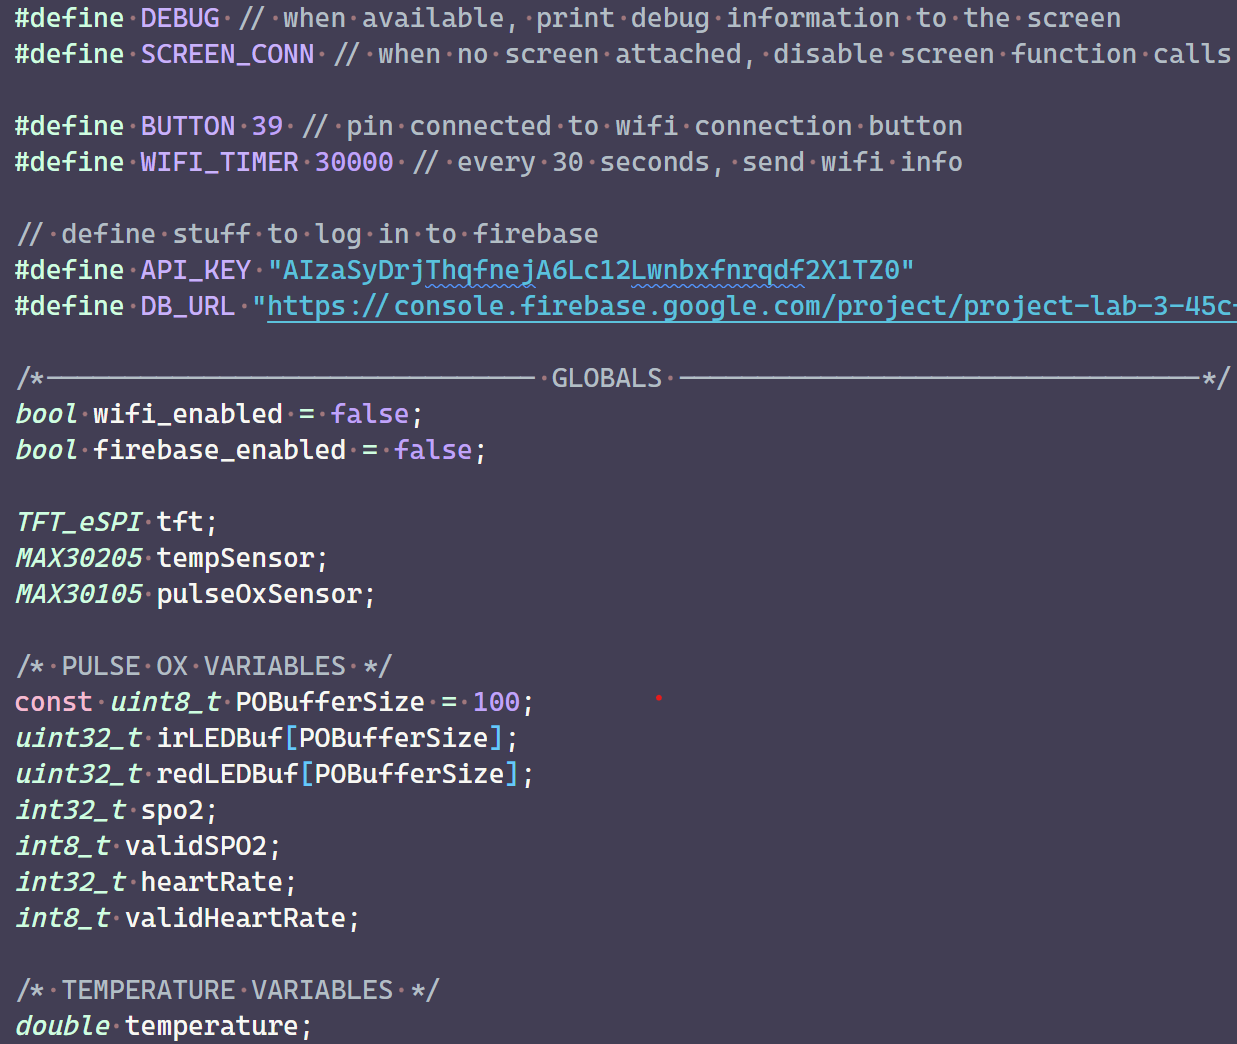
\includegraphics[width=0.75\textwidth]{uc_globals}
        \caption{Microcontroller - Global Variables Snippet}
        \label{uc_var}
    \end{figure} 

    \begin{figure}[ht]
        \centering
        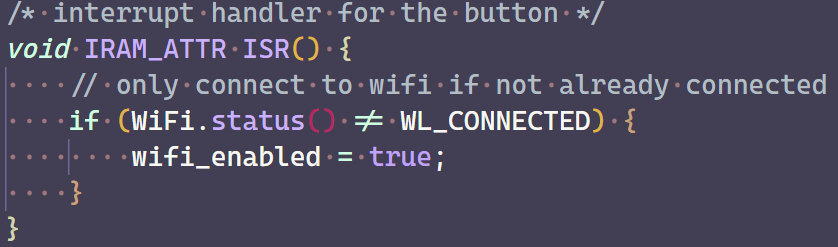
\includegraphics[width=0.75\textwidth]{uc_isr}
        \caption{Microcontroller - Interrupt Service Routine}
        \label{uc_isr}
    \end{figure} 

    To clean up the code, two helper functions were written in order to assist. The first function simply converts a temperature in Celsius to Fahrenheit, this is done for the body temperature sensor, as body temperature in Celsius is less useful for humans than in Fahrenheit. The second function sets up WiFi when triggered from a button press in the main loop. First, the flag which triggered the function is disabled to ensure it doesn't trigger unnecessarily again. Then, an instance of the WiFiManager object is declared and called to connect to the WiFi. This happens by starting the ESP32 as its own access point, then a user device like a phone can login to the ESP32 and define a WiFi connection for it to talk to on its own \cite{wifi_manager}. After that is setup, the ESP32 automatically switches over to a device, where it then connects to the given network and works as expected. Both functions are shown in Figure \ref{uc_help}.

    \begin{figure}[ht]
        \centering
        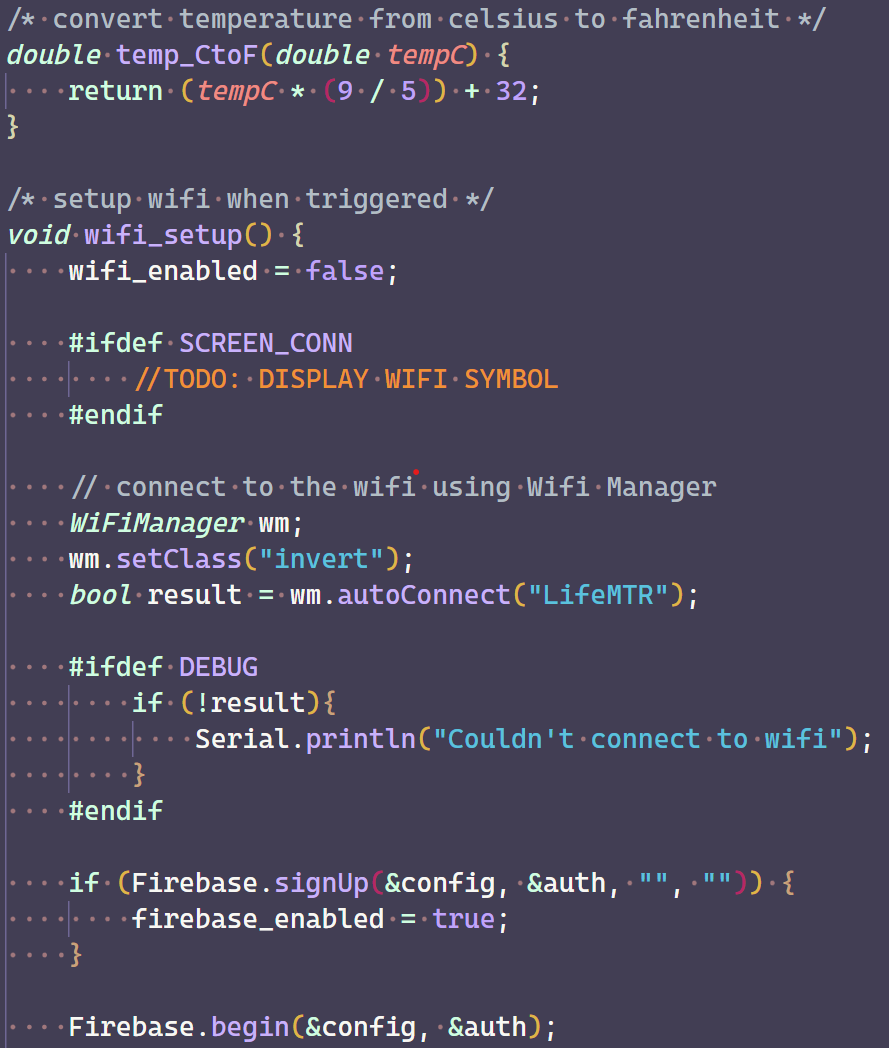
\includegraphics[width=0.75\textwidth]{uc_helpers}
        \caption{Microcontroller - Helper Functions}
        \label{uc_help}
    \end{figure} 

    The main setup function initializes several components and the global variables. First, the Firebase API keys and URL are put into a global config object for the Realtime Database \cite{firebase_client_lib}. If the debug flag is currently active, the code also sets up a serial connection to the PC the ESP32 is connected to. If the screen is connected, it then initializes the TFT\_eSPI screen and displays a boot logo. The code then sets up both of the sensors, the MAX30205 temperature sensor and the MAX30102 pulse oximeter with the ESP32's I2C bus \cite{protocentral_max30205,sparkfun_max301x}. The temperature sensor setup is a quick check to make sure it is there, however the pulse oximeter requires a more in depth process as described by the datasheet. When first booted, the sensor should run through a full reading, as its first measurement is not correct due to outside factors and calibration \cite{max30102}. Finally, the setup is finished after setting up the button with an internal pull-up resistor and attaching an interrupt to that pin, which allows the ESP32 to fire the ISR if pressed. This functionality is shown in Figure \ref{uc_setup}.

    \begin{figure}[ht]
        \centering
        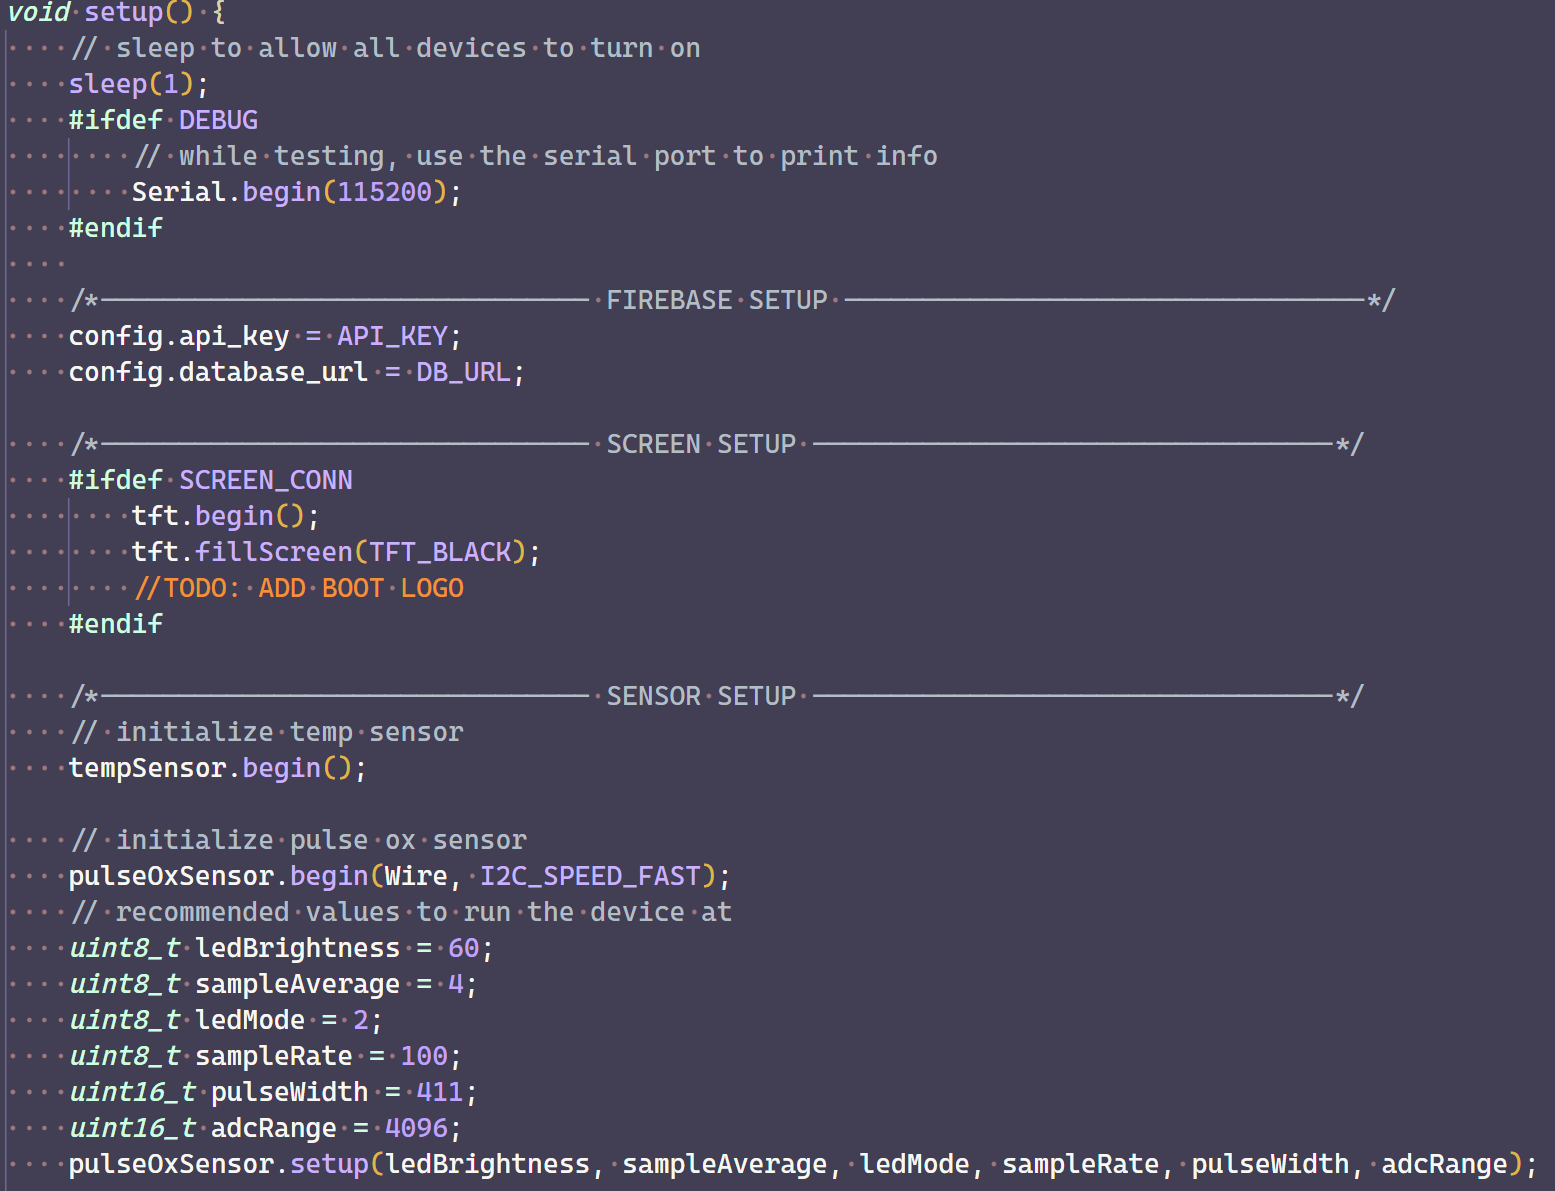
\includegraphics[width=0.6\textwidth]{uc_setup}
        \caption{Microcontroller - Setup Snippet}
        \label{uc_setup}
    \end{figure} 

    The loop function is the main code loop. Every iteration, the pulse oximeter is triggered to take a new 25 samples using the same code as shown above in the setup. The temperature sensor also takes a reading each time, which then is immediately converted to Fahrenheit for later use. If the debug is active, the current values of different registers are displayed on the screen, just for the developer to ensure the sensors are working properly. This part of the code is also what is checking for the WiFi flag to be triggered, which it will then decide to setup WiFi or just to ignore it. This prevents any spurious button clicks to do anything detrimental to the running of the device. Finally, the loop checks every 30 seconds if WiFi is connected and Firebase is properly configured, if it is it asynchronously sends the values to the Firebase server \cite{firebase_client_lib}. This function is shown in Figure \ref{uc_main}.

    \begin{figure}[ht]
        \centering
        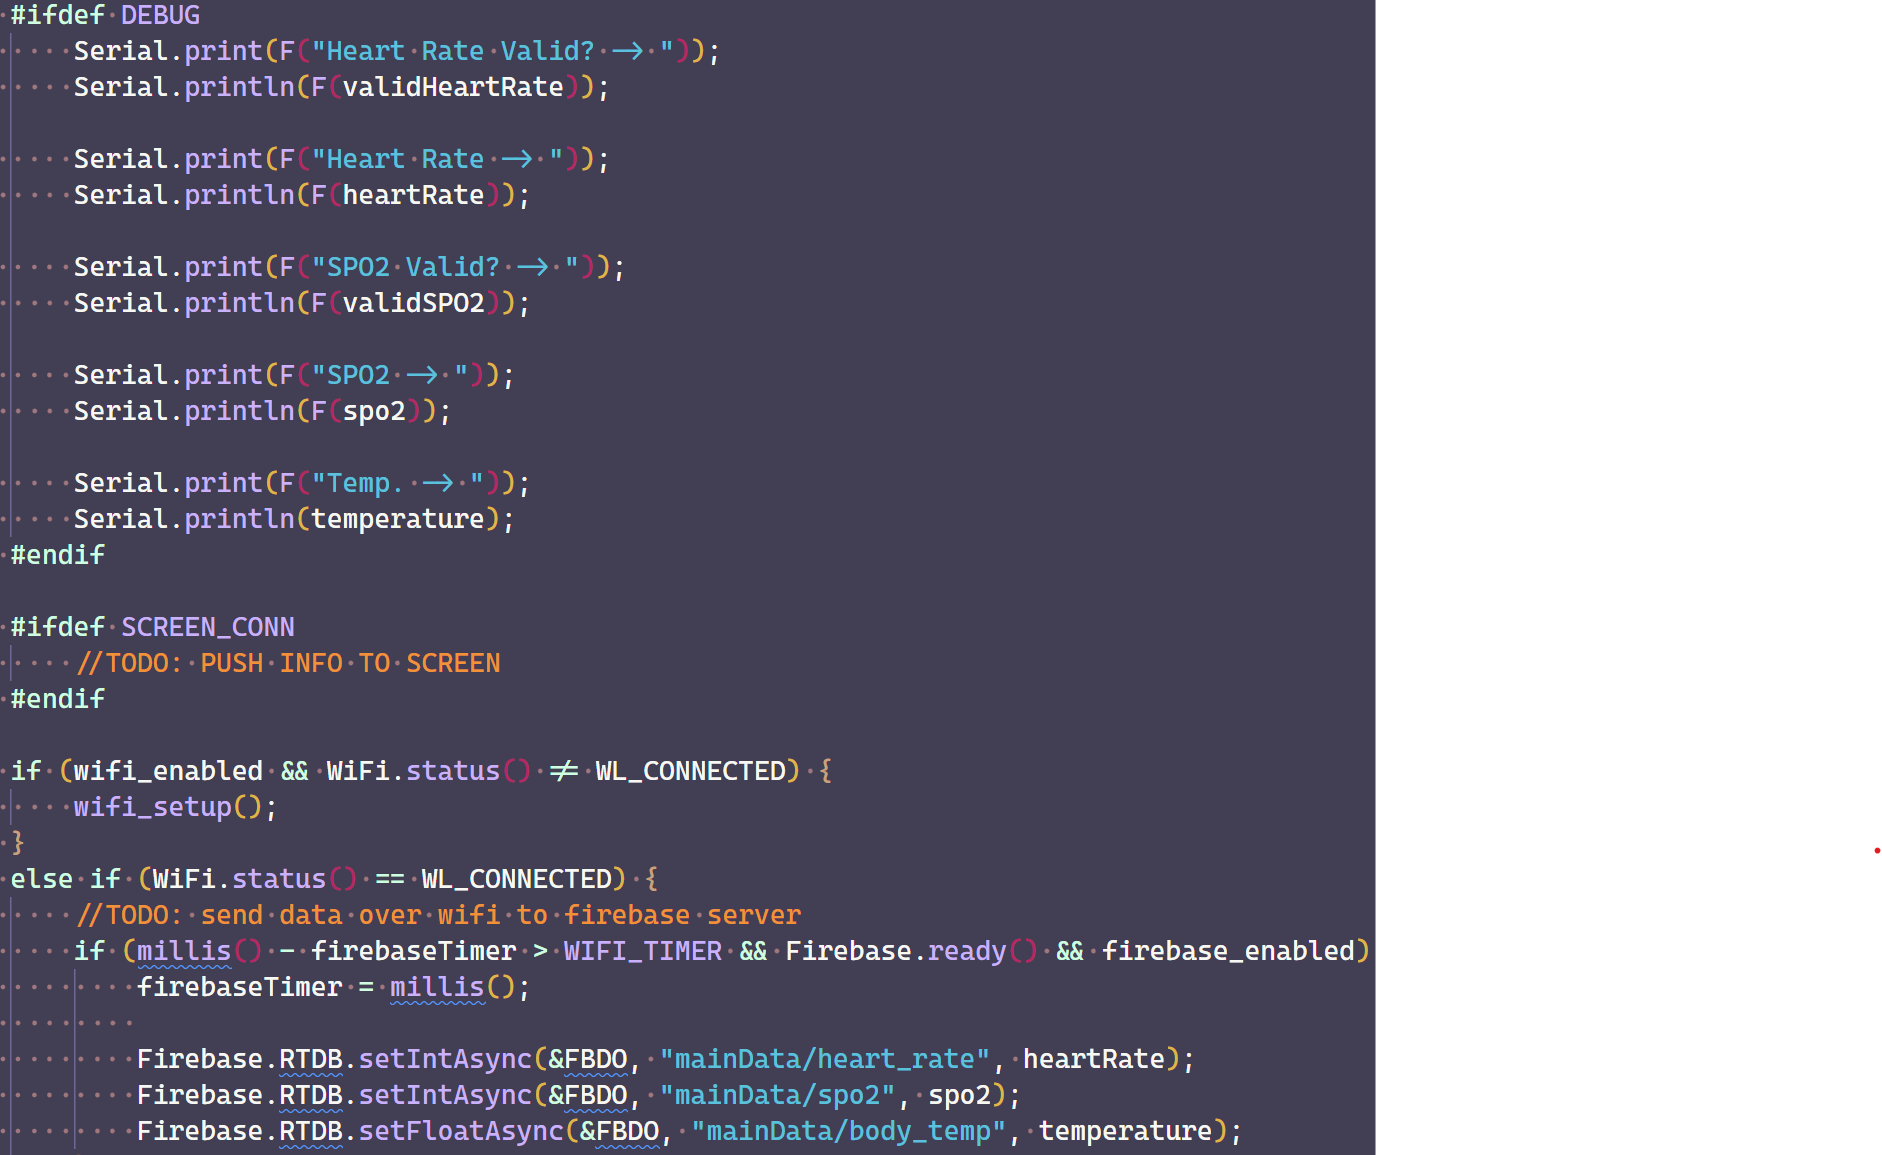
\includegraphics[width=0.6\textwidth]{uc_main}
        \caption{Microcontroller - Main Loop Snippet}
        \label{uc_main}
    \end{figure} 

    \subsubsection{Firebase}
    To store and display the data received from the device, a Firebase backend is utilized as a simple yet powerful tool to to manage the database and to host the website. The main database being used is a Realtime Database, which is an asynchronous database that automatically updates as data arrives, which is different than a standard database that updates based on HTTP requests \cite{firebase}. The database is accessed through the Firebase Client deployed onto the ESP32, which sends the heart rate, the blood oxygen level, and the body temperature to the mainData node, which holds space for each data type. The organization of the database is shown in Figure \ref{fb_struct}. The database is based on NoSQL, and each variable in the data is a JSON variable, which makes for easier modification and lightweight packets to send \cite{firebase}. 

    \begin{figure}[ht]
        \centering
        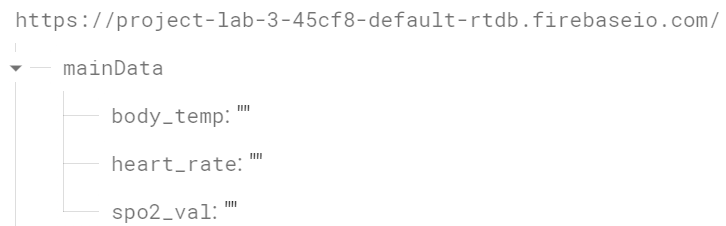
\includegraphics[width=0.75\textwidth]{firebase_structure}
        \caption{Firebase - Database Structure}
        \label{fb_struct}
    \end{figure} 

    Firebase is also used to host a website based on JavaScript which contains a pleasant landing page for the user to access. This page is shown in Figure \ref{fb_website}. The other page is the visualization of the database, with a graph for time and the three variables.  This is shown in Figure \ref{fb_data}.

    \begin{figure}[ht]
        \centering
        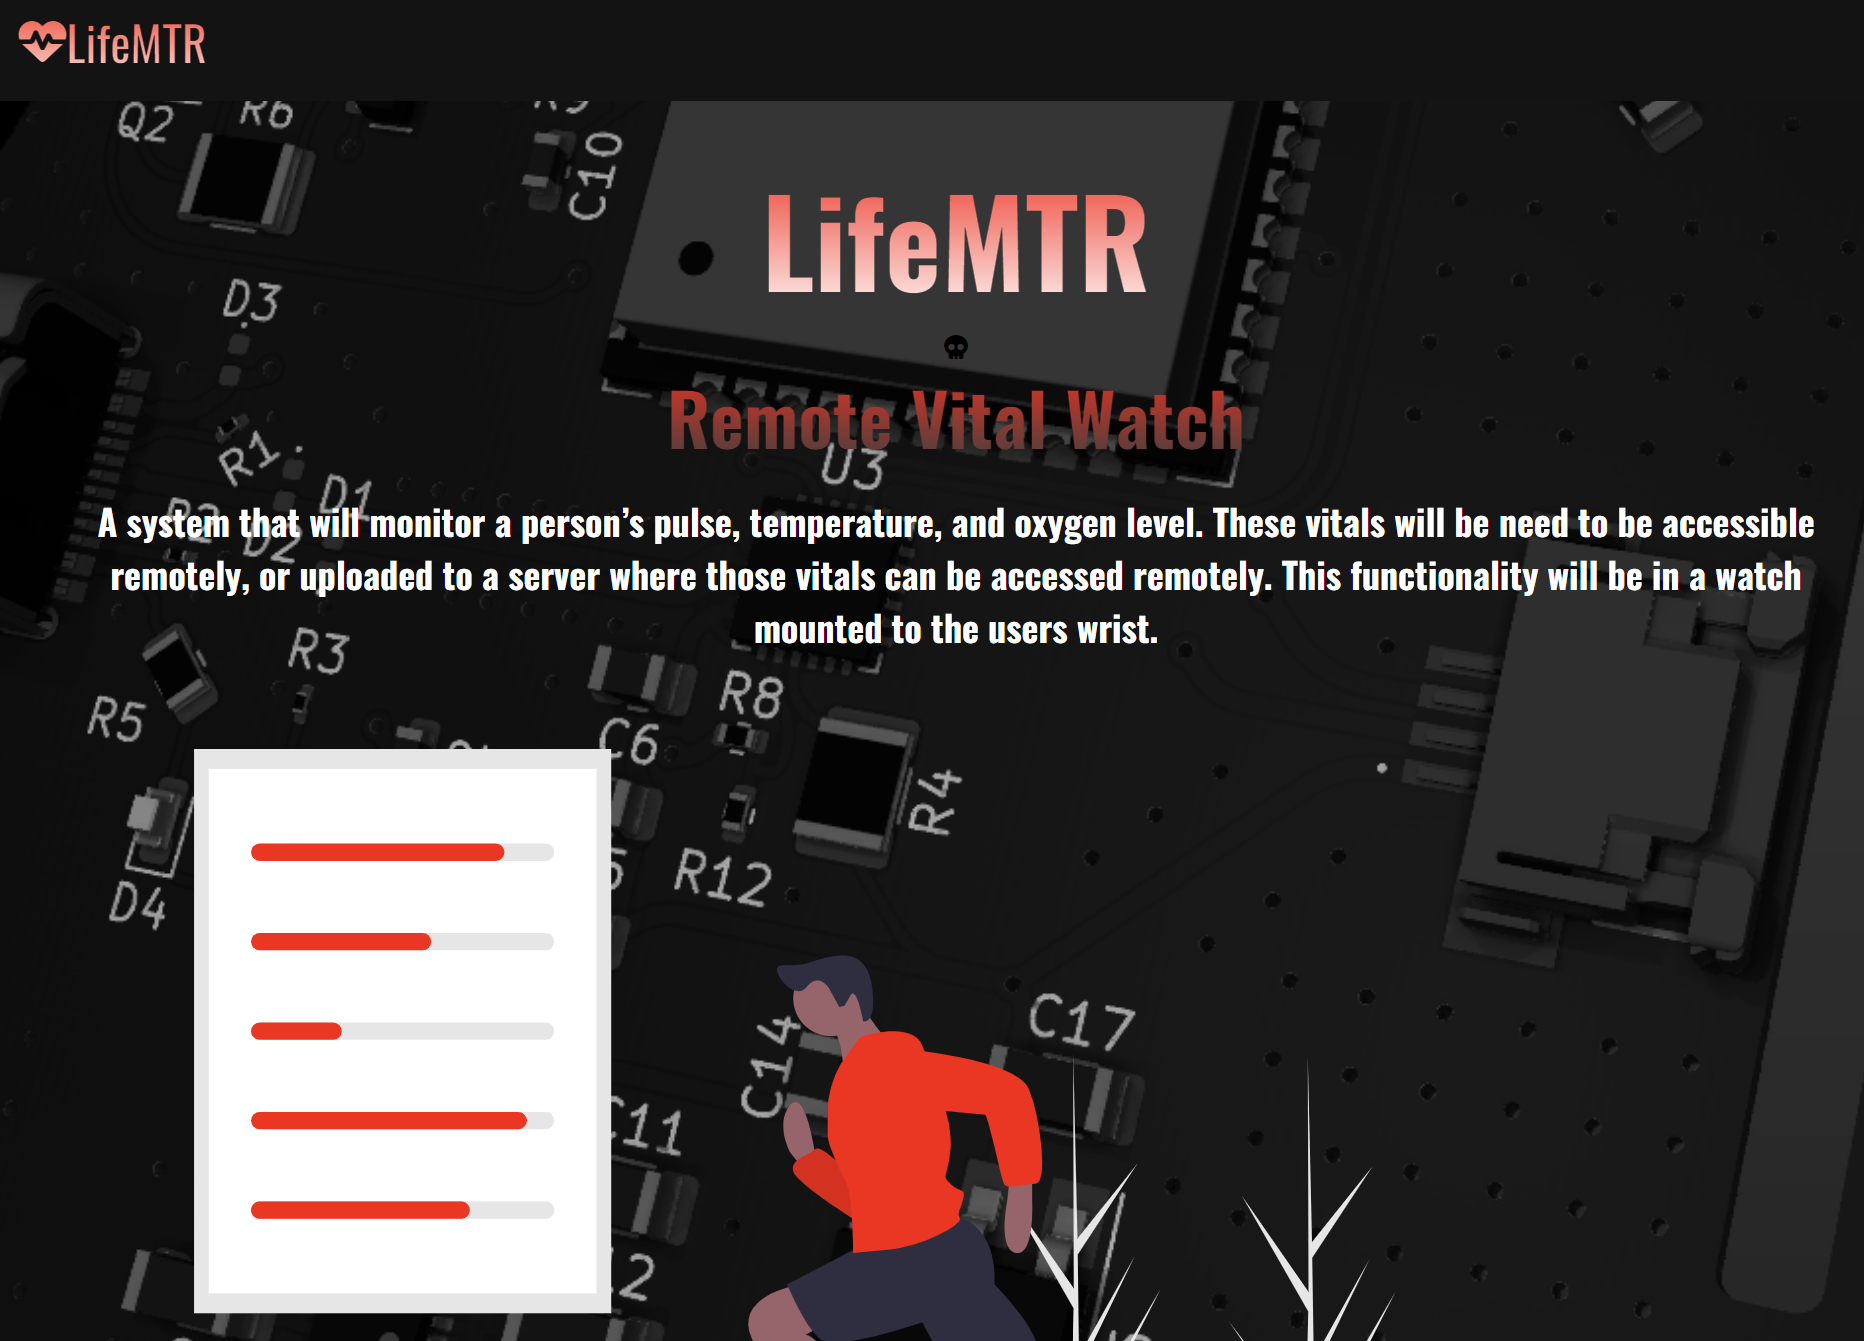
\includegraphics[width=0.75\textwidth]{images/fb_website.png}
        \caption{Firebase - Website Main Page}
        \label{fb_website}
    \end{figure} 

    \begin{figure}[ht]
        \centering
        
\includegraphics[width=0.75\textwidth]{images/fb_data.png}
        \caption{Firebase - Website Data Display}
        \label{fb_data}
    \end{figure} 

\subsection{Hardware}
\subsubsection{Motherboard PCB}
    The motherboard PCB consists of five sections, the USB input and UART, the battery charging circuit, the power supply, the microcontroller, and the output. The USB input provides power for the battery charging circuit and sends data to the USB to UART chip for programming. A USB 2.0 USB C connector is used for the power and data lines, as the extra complexity of USB 3.0 or greater does not affect the data transfer times while adding much more components and routing effort. ESD321 TVS diodes are placed on the two data lines and the power input line for electrostatic discharge protection due to a person plugging in the cable. The data lines are impedance matched to 90 $\Omega$, which is required of the USB 2.0 standard to ensure proper data transfer \cite{usb_spec}. 5.1 K$\Omega$ configuration resistors are used to tell the device to only draw as much current as is being used. This part of the circuit is shown in Figure \ref{pcb_usb}.

    \begin{figure}[ht]
        \centering
        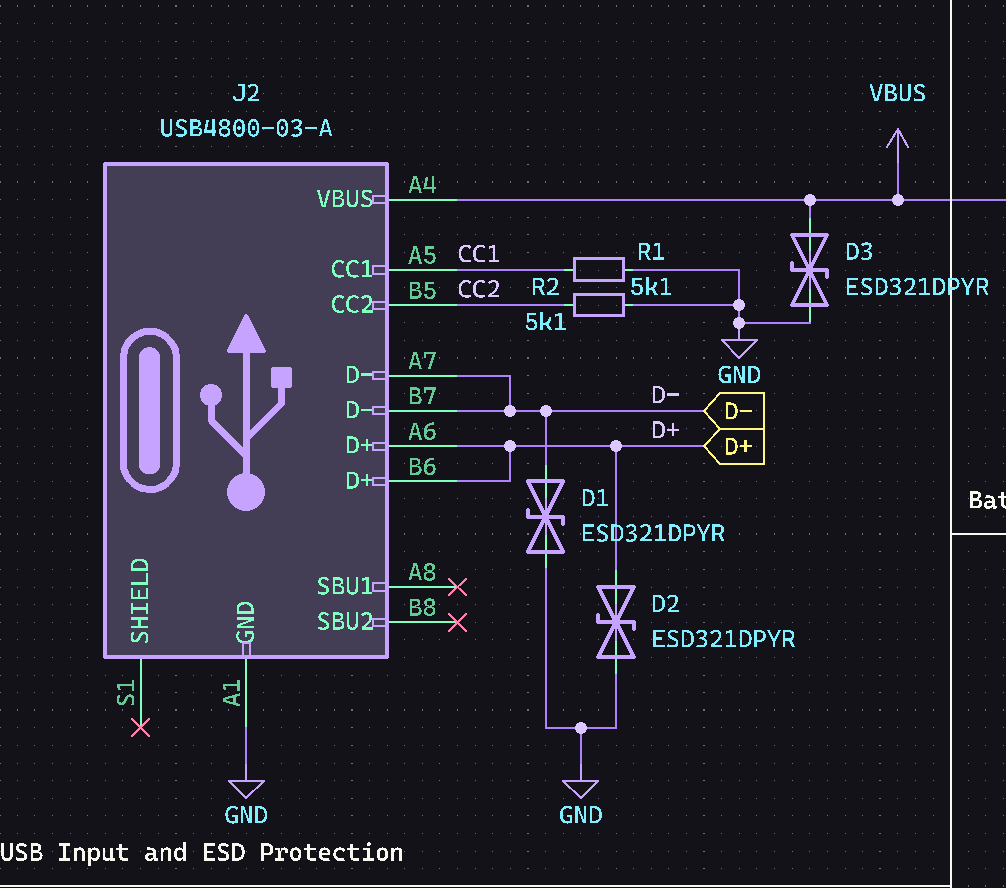
\includegraphics[width=0.6\textwidth]{images/pcb_usb.png}
        \caption{Motherboard - USB Input}
        \label{pcb_usb}
    \end{figure}

    The battery charging circuit is powered by the MCP7382T battery charging IC \cite{mcp73832}. The positive input of the battery is connected to the VBAT pin on the chip, which provides charging based on the chosen resistor, in this case a 2.2 K$\Omega$ resistor that sets the the output current to 450mA. 450mA is chosen as the charge current because the battery is a 500 mAH LiPo battery, so the charge current should be a little less than the full amount for safety reasons. The circuit also consists of various decoupling and bypass capacitors. The circuit is shown in Figure \ref{pcb_battery}.

    \begin{figure}[ht]
        \centering
        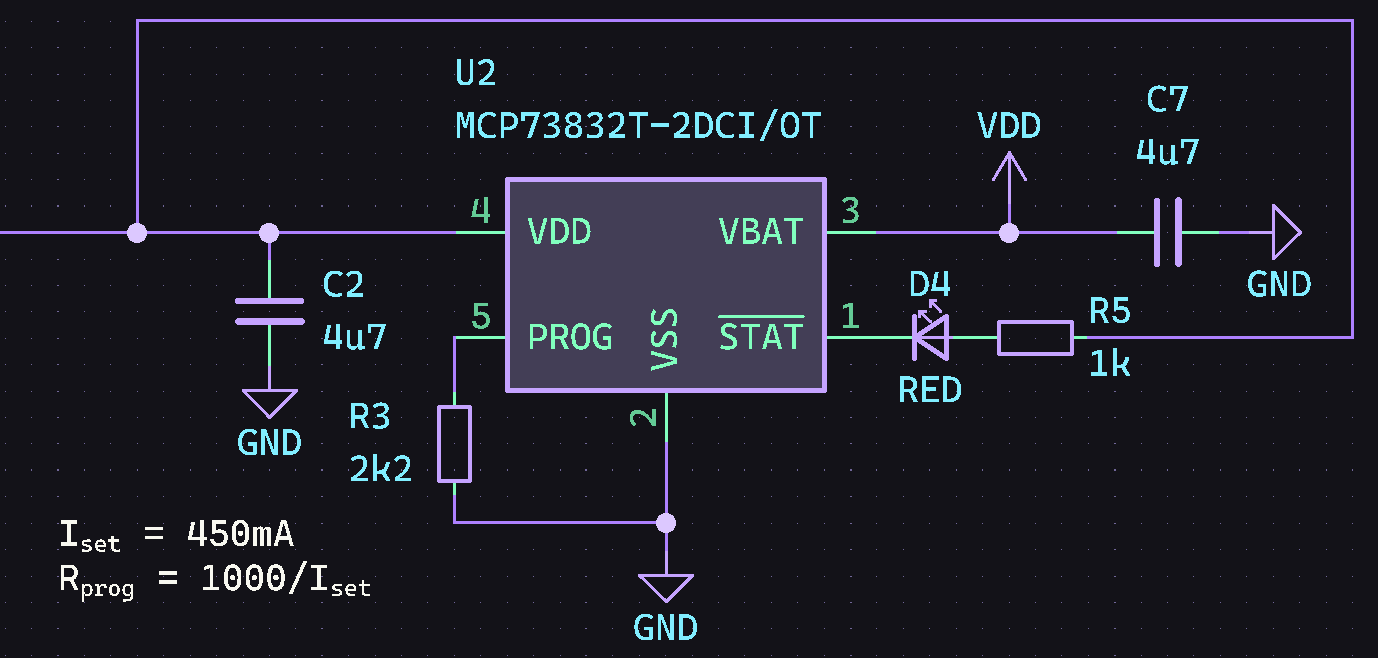
\includegraphics[width=0.6\textwidth]{images/pcb_battery.png}
        \caption{Motherboard - Battery Charging Circuit}
        \label{pcb_battery}
    \end{figure}

    The next circuit on the board is the multi-stage power supply. The first stage is a boost converter powered by the TPS61230DRC boost converter \cite{boost}. This brings the varying range of the battery voltage to a constant 5V, which is useful to power the microcontroller. The voltage needs to remain at this higher state for the following component, an AZ1117IH-3.3TRG1 3.3V low dropout regulator \cite{3v3}. This regulator drops the 5V to 3.3V which is what the microcontroller and the peripherals use. Like before, the circuits also contain the various decoupling capacitors and inductors and feedback resistors on the boost converter to set the voltage. This is shown in Figure \ref{pcb_power}.

    \begin{figure}[ht]
        \centering
        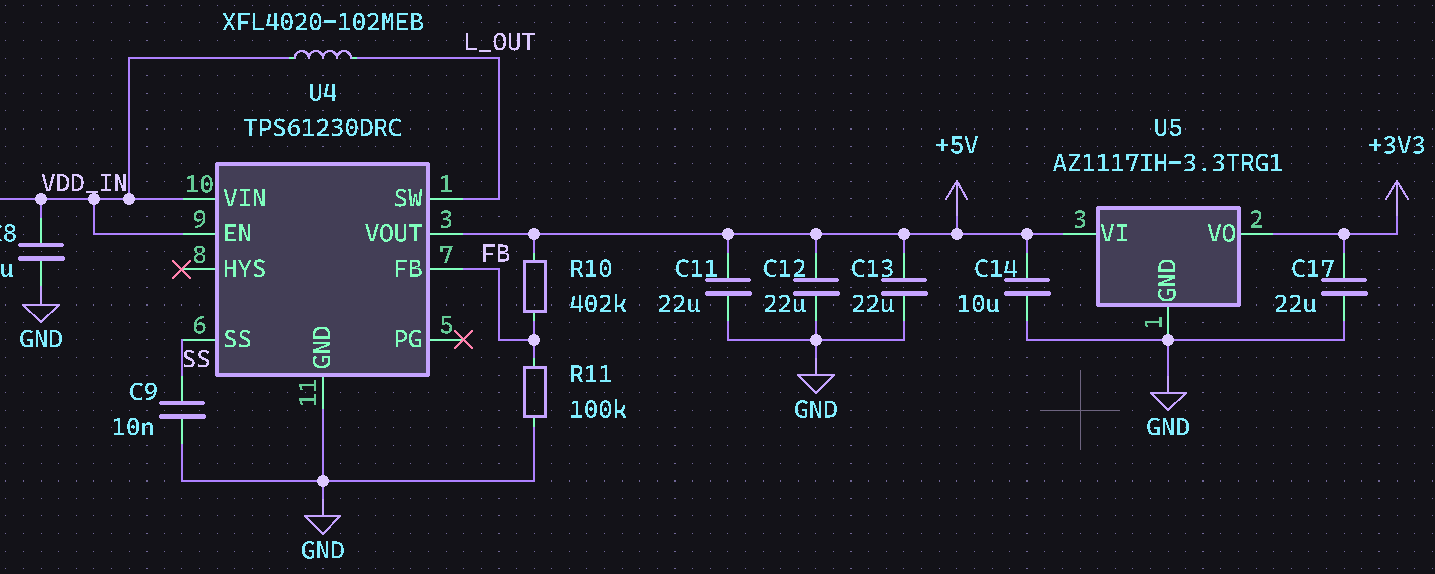
\includegraphics[width=0.6\textwidth]{images/pcb_power.png}
        \caption{Motherboard - Multi-Stage Power Supply}
        \label{pcb_power}
    \end{figure}

    The main section of the circuit is the microcontroller and the UART converter chip. The ESP32 is relatively simple to build a circuit for \cite{esp32}, requiring only a few resistors and capactitors to make an RC circuit for booting and flashing. The ESP32 also has a setup of NPN transistors which allow the device to automatically set the boot and IO0 pins at the correct levels based on the output of the control signals on the UART chip \cite{esp32, UART}. The CP2102N is slightly more complicated to create a circuit for, however it is just a few resistors and decoupling capacitors. The CP2012N and the programming circuit are shown in Figure \ref{pcb_uart}, and the circuit for the ESP32 is shown in Figure \ref{pcb_esp32}.

    \begin{figure}[ht]
        \centering
        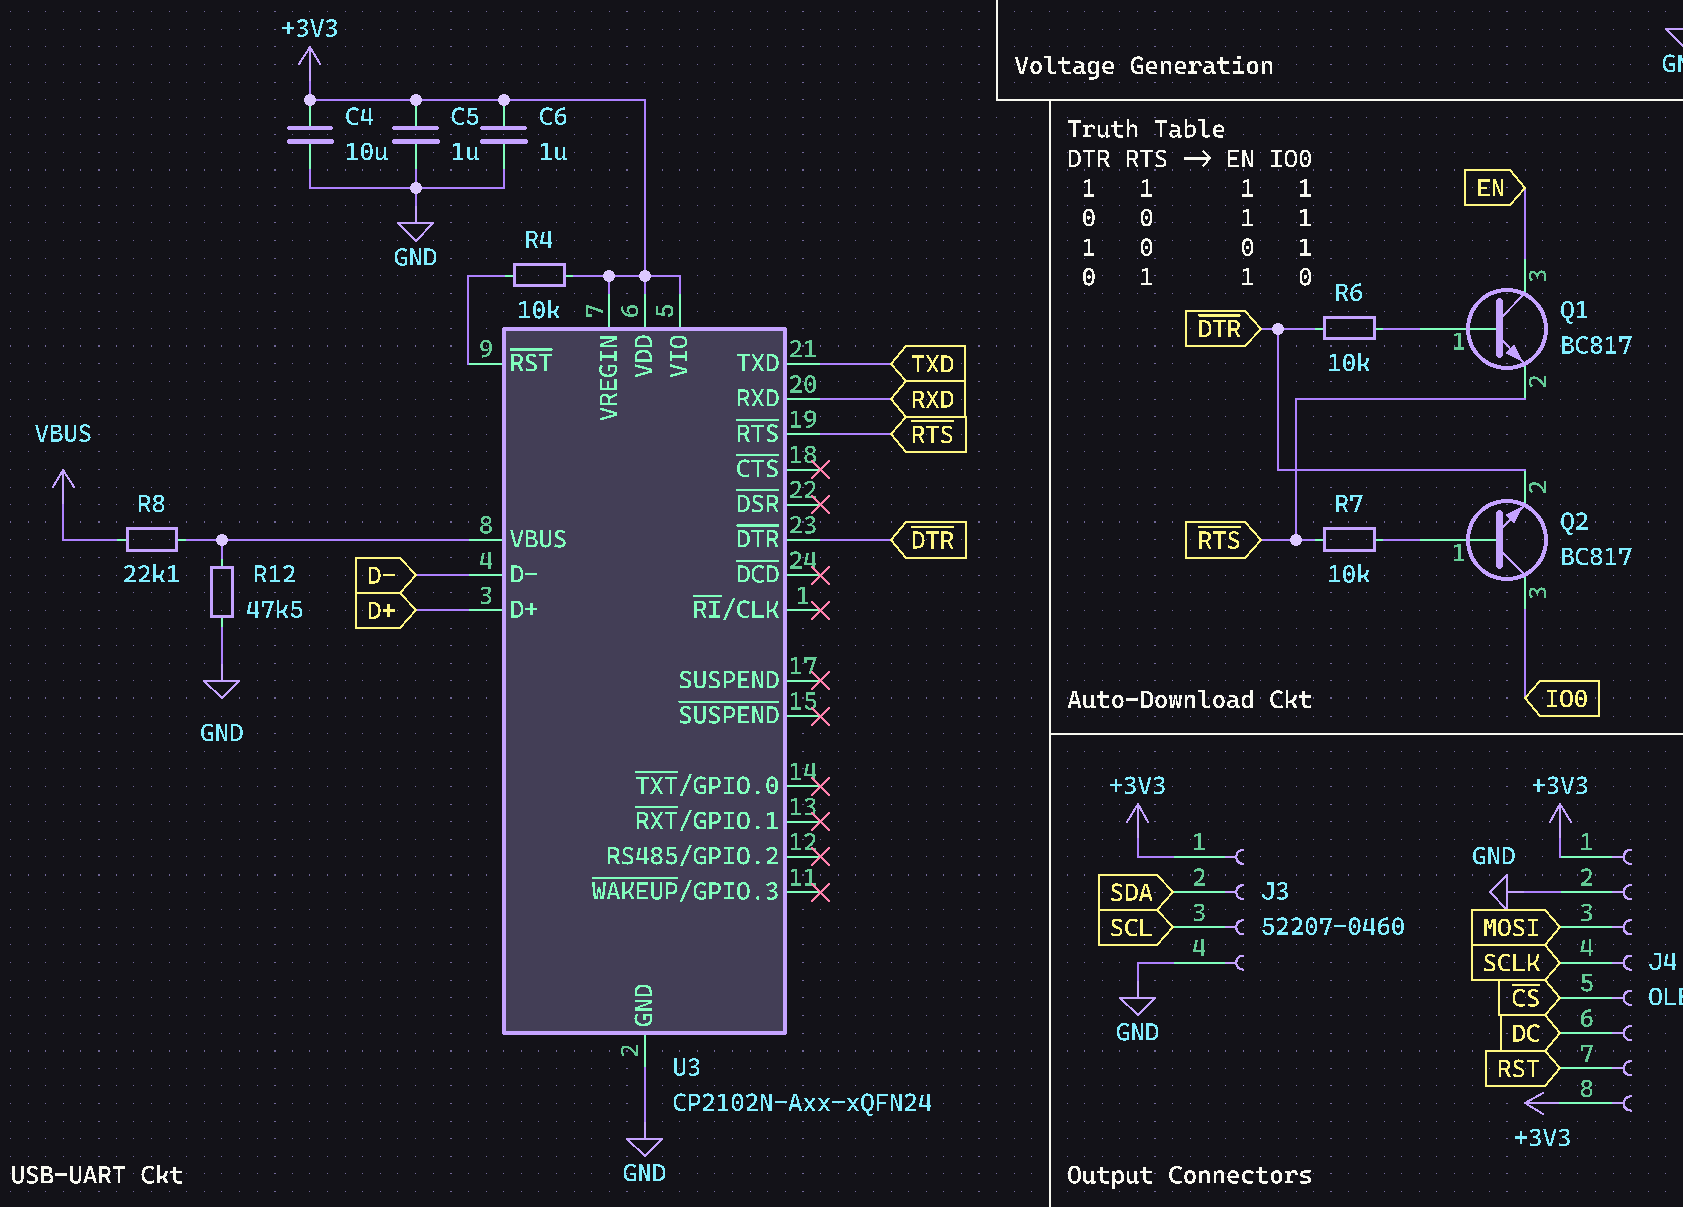
\includegraphics[width=0.6\textwidth]{images/pcb_uart.png}
        \caption{Motherboard - USB to UART Circuit}
        \label{pcb_uart}
    \end{figure}

    \begin{figure}[ht]
        \centering
        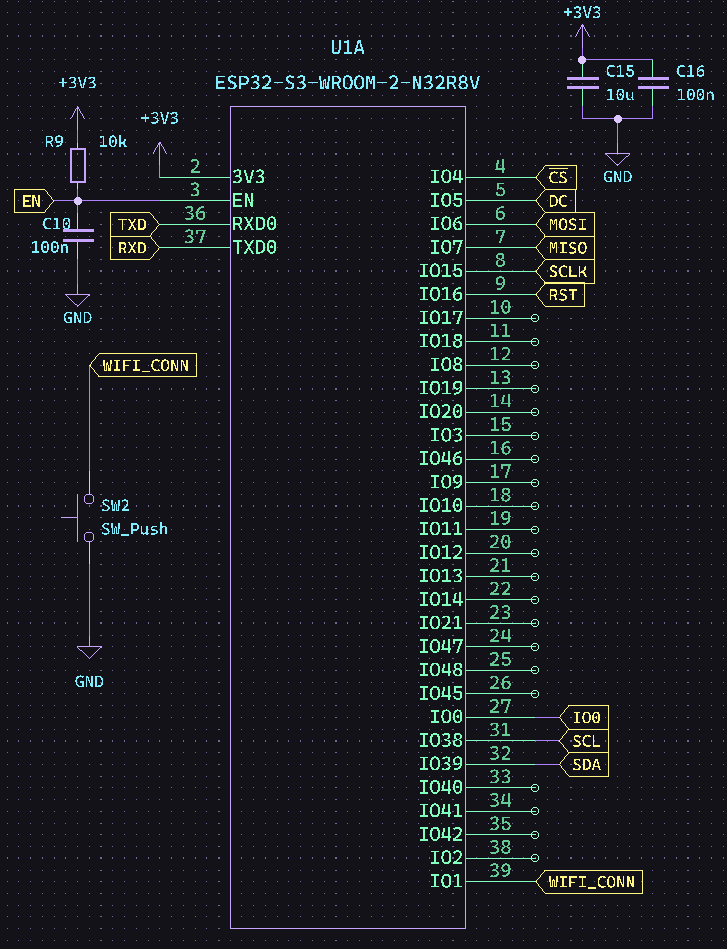
\includegraphics[width=0.6\textwidth]{images/pcb_esp32.png}
        \caption{Motherboard - ESP32}
        \label{pcb_esp32}
    \end{figure}

    The final routing of the board is simply a combination of datasheet recommendations and common sense layout recommendations, such as ensuring proper grounding, making sure traces are wide enough for the anticipated current, and not mixing high frequency signals with high power signals. A circle was decided as the shape for the board as the final design was originally meant to be a watch, however due to size it was decided that a chest mounted design like the arc reactor from Iron Man would be more functional than an oversized arm piece. The final board is shown in Figure \ref{pcb_board}. The output, which is pictured in Figure \ref{pcb_uart}, is a flat ribbon cable which allows I2C signals to be sent between the ESP32 and the daughter-board, which will be further discussed next.

    \begin{figure}[ht]
        \centering
        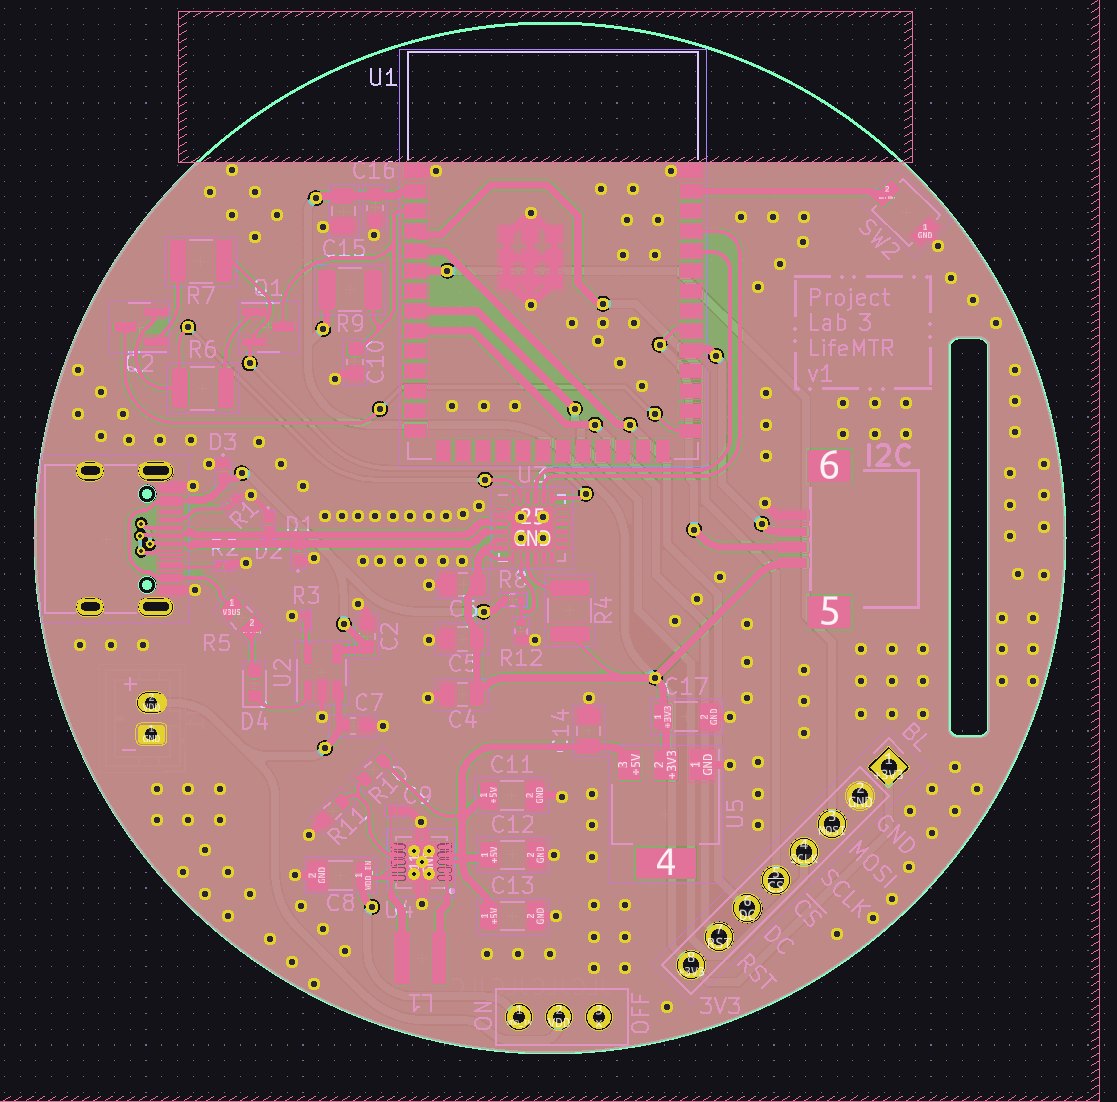
\includegraphics[width=0.6\textwidth]{images/pcb_board.png}
        \caption{Motherboard - Full Board}
        \label{pcb_board}
    \end{figure}

    \subsubsection{Daughter-board PCB}
    The daughter-board is used to allow the sensors that require skin contact to remain in good contact with the skin regardless of the enclosure and other parts used. The top side of the board contains a regulator and general resistors and decoupling capacitors for the two sensor ICs which are on the bottom. The main IC on the top half of the board is the ADP7182AUJZ-1.8, a 1.8V low dropout regulator to power the MAX30102 chip and its LEDs \cite{1v8}. The top of the board also contains 4.7 K$\Omega$ resistors for the I2C lines, and a handful of decoupling capcitors. The bottom of this board contains the sensor ICs for pulse oximetry, heart rate, and body temperature. Figure \ref{db_schem} shows the schematic of the board, and Figure \ref{db_board} shows the layout of the board.
    
    \begin{figure}[ht]
        \centering
        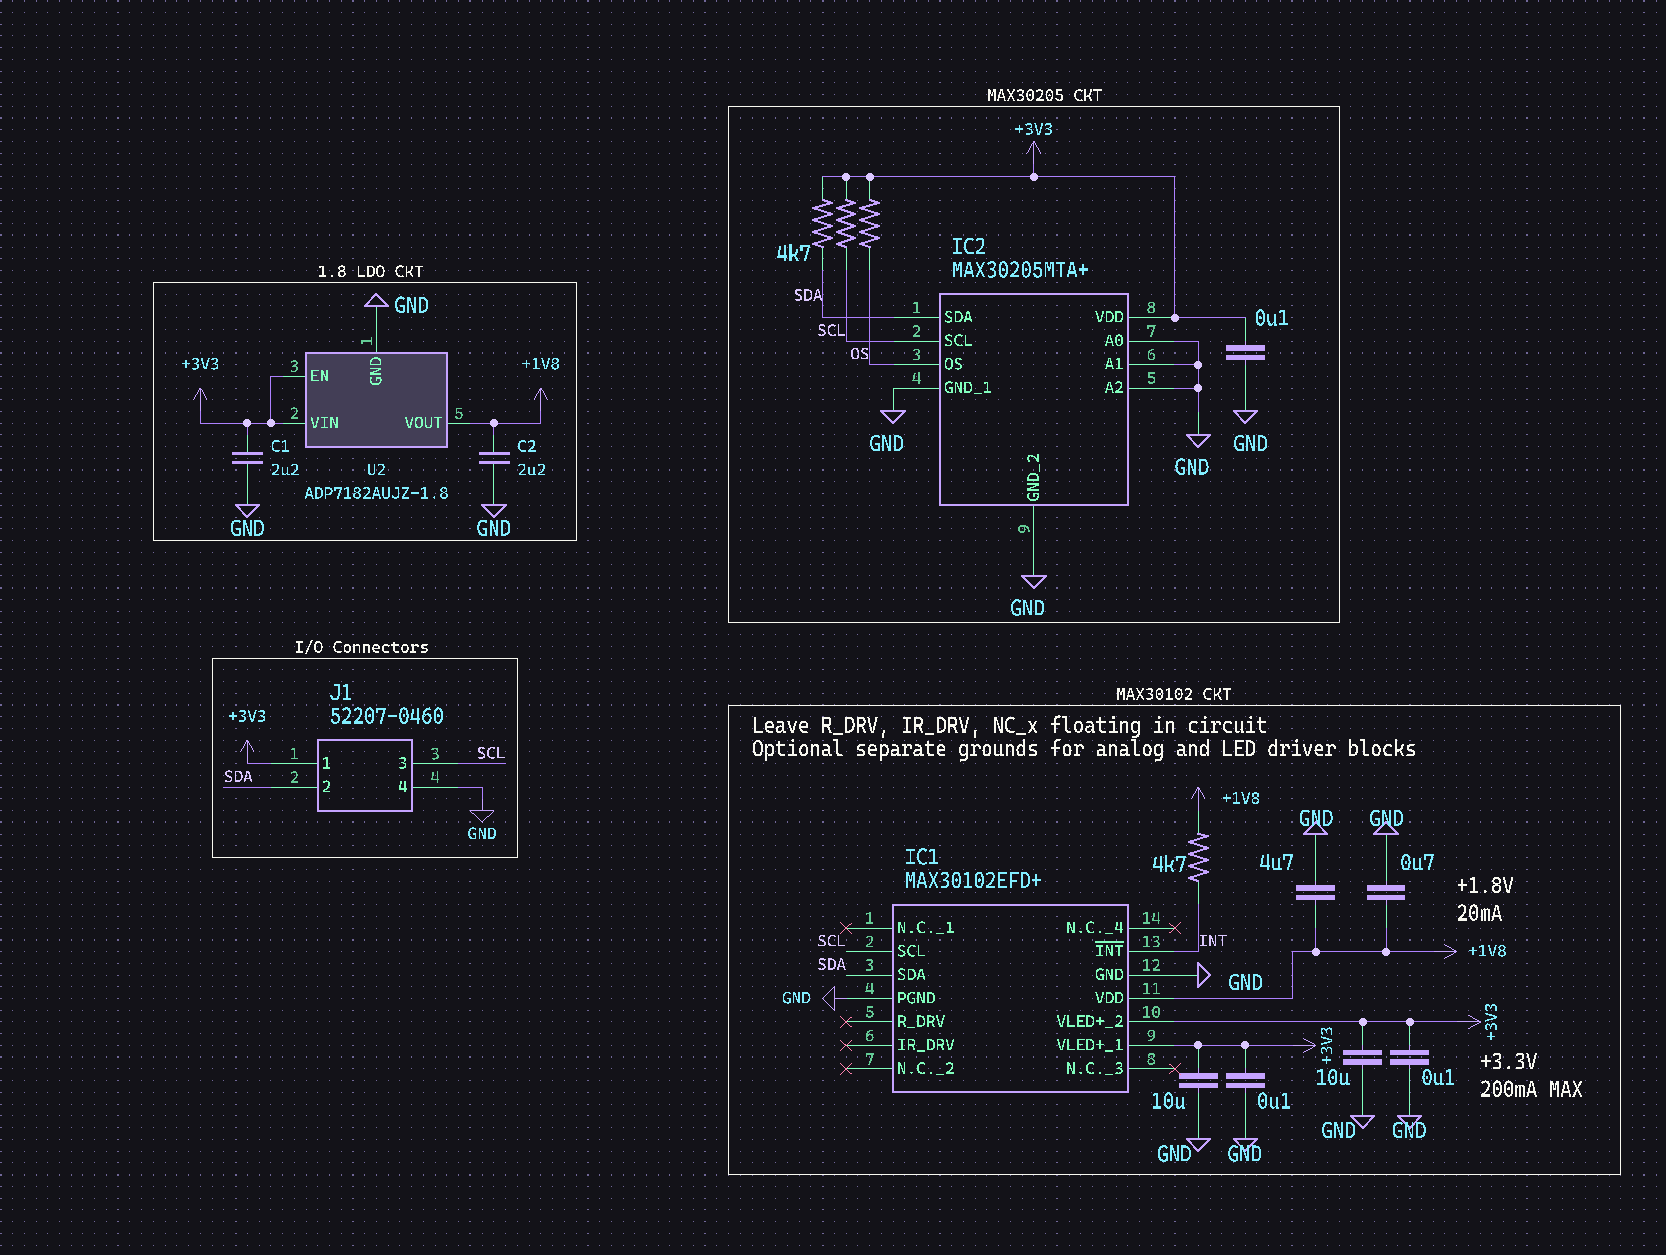
\includegraphics[width=0.6\textwidth]{images/mb_schematic.png}
        \caption{Daughter-Board - Schematic}
        \label{db_schem}
    \end{figure}

    \begin{figure}[ht]
        \centering
        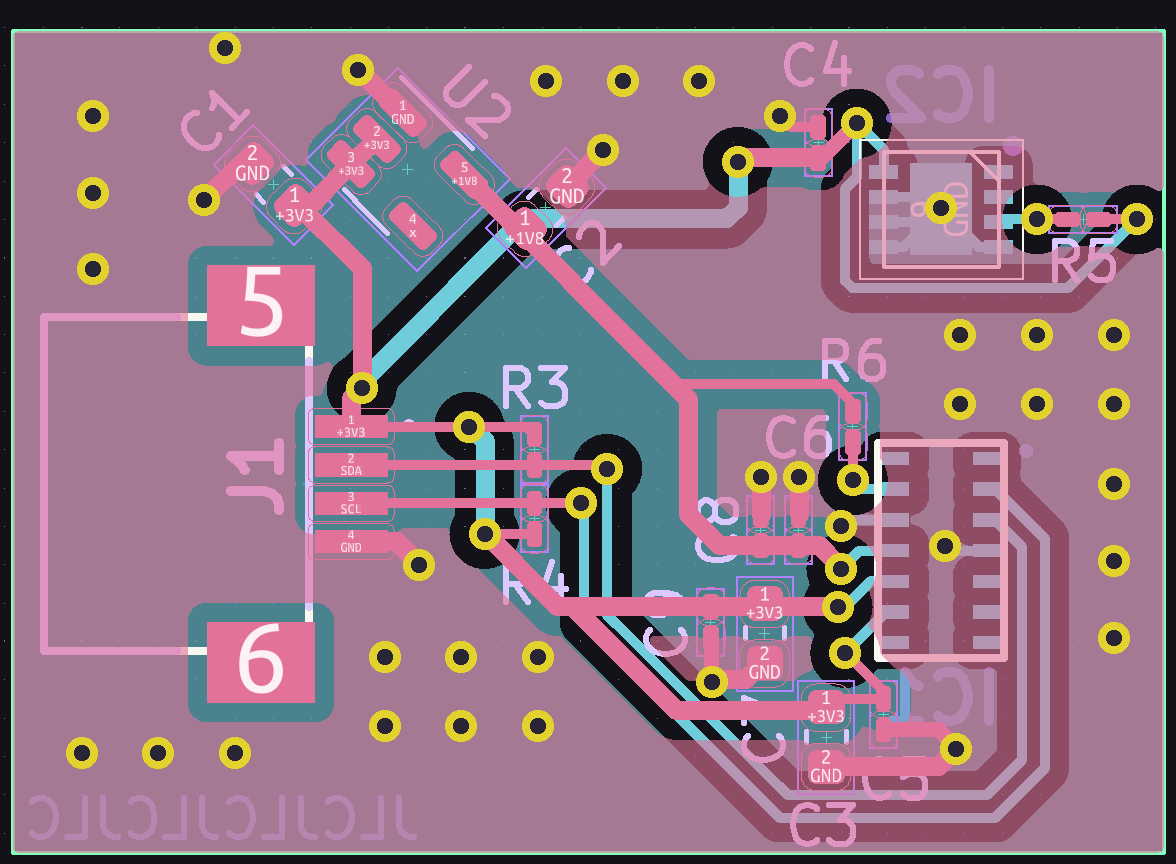
\includegraphics[width=0.6\textwidth]{images/mb_board.png}
        \caption{Daughter-Board - Board}
        \label{db_board}
    \end{figure}

\section{Conclusion}
    While the project isn't currently finished, much of the required progress has been completed. The main PCBs are currently assembled and nearly ready to go, with only a few shorts to clean up and make good. The code is about 90\% finished and is ready for testing on a pre-made ESP32. Software debouncing will be added to th ISR code to prevent an accidental button presses, but right now the current iteration the code is not debouncing any button presses. The final enclosure needs to be designed to fit all the boards and the battery chosen. As stated previously, the battery is currently a 500 mAH, however, a larger battery may be chosen due to the fact that there is now more space available.

\newpage
\newpage
\section{Appendix}
\subsection{GANTT Chart and Budget}
\begin{figure}[ht]
    \centering
    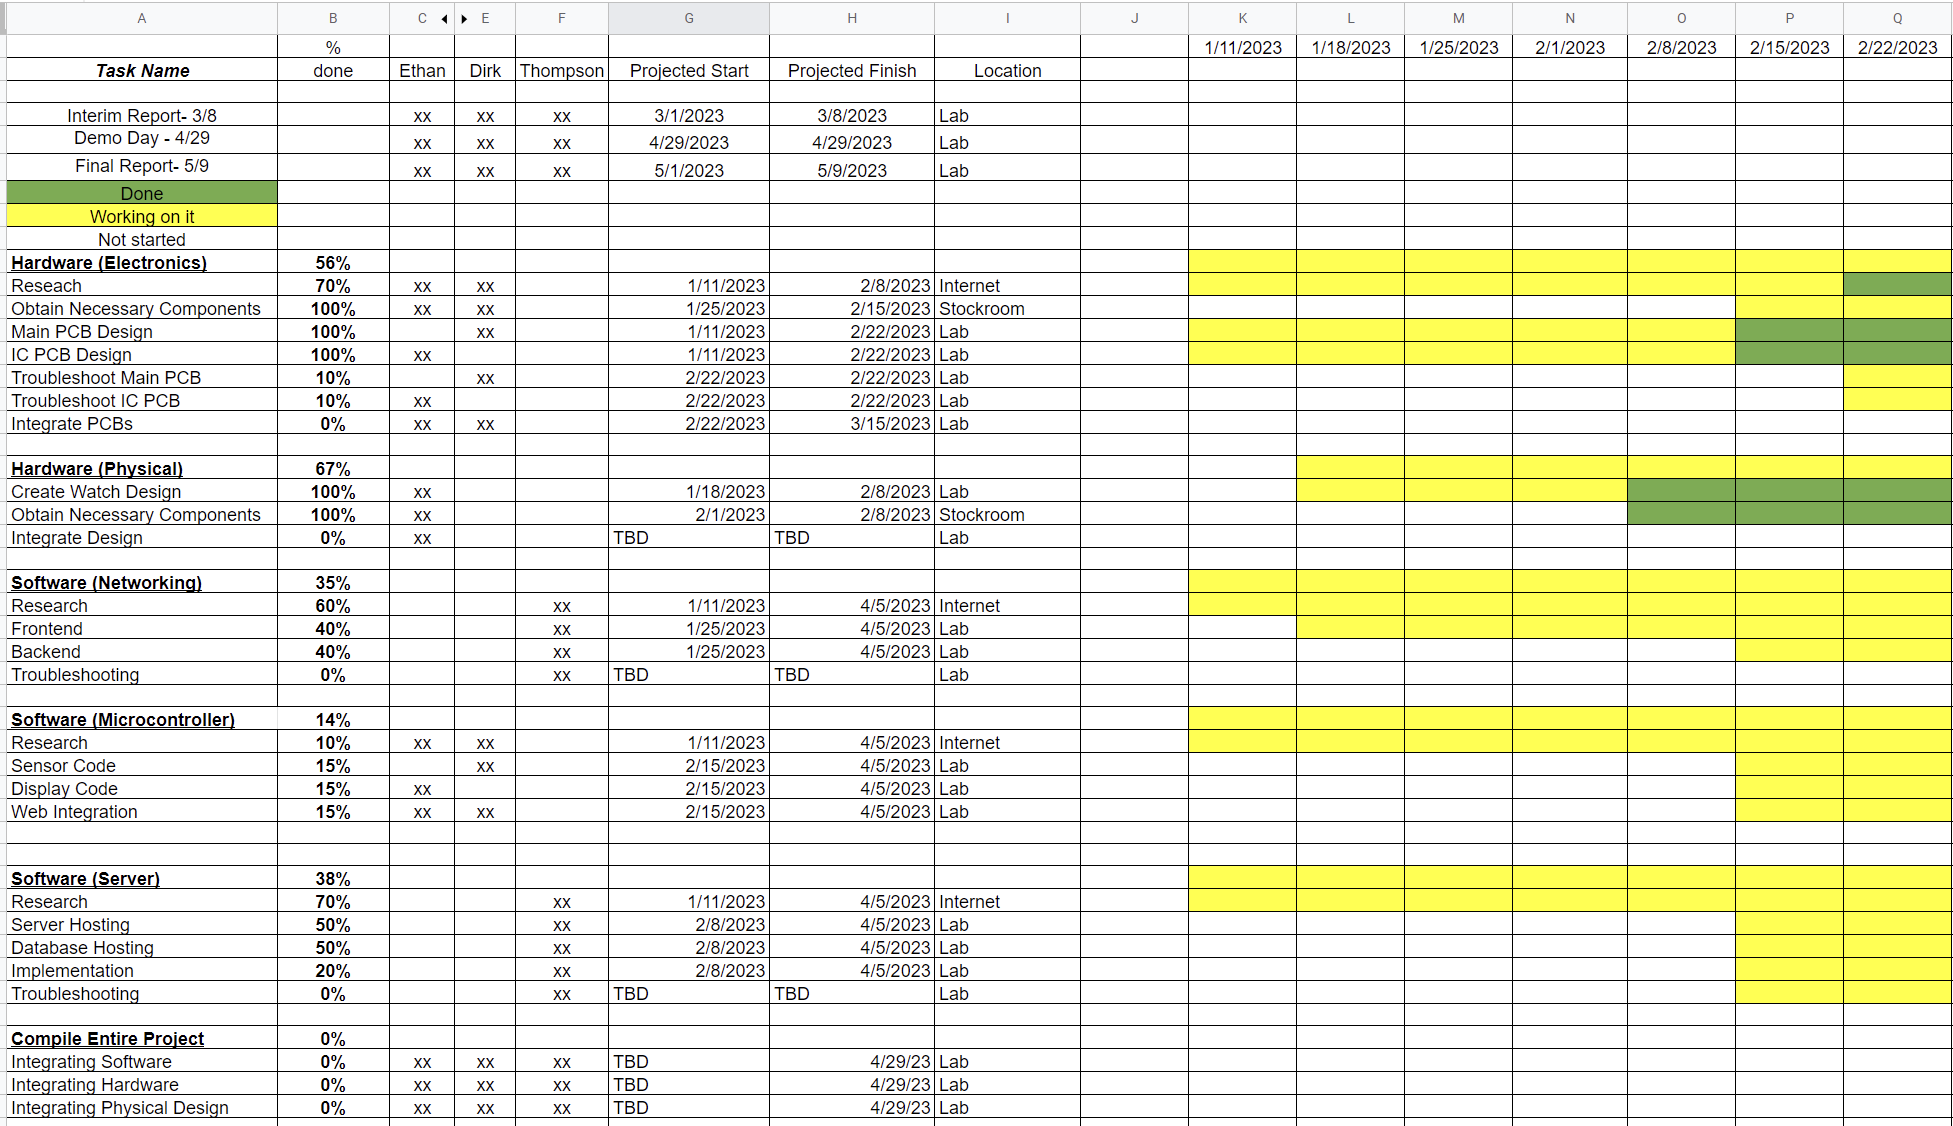
\includegraphics[width=0.75\textwidth]{images/gantt.png}
    \caption{GANTT Chart}
    \label{gantt}
\end{figure}

\begin{figure}[ht]
    \centering
    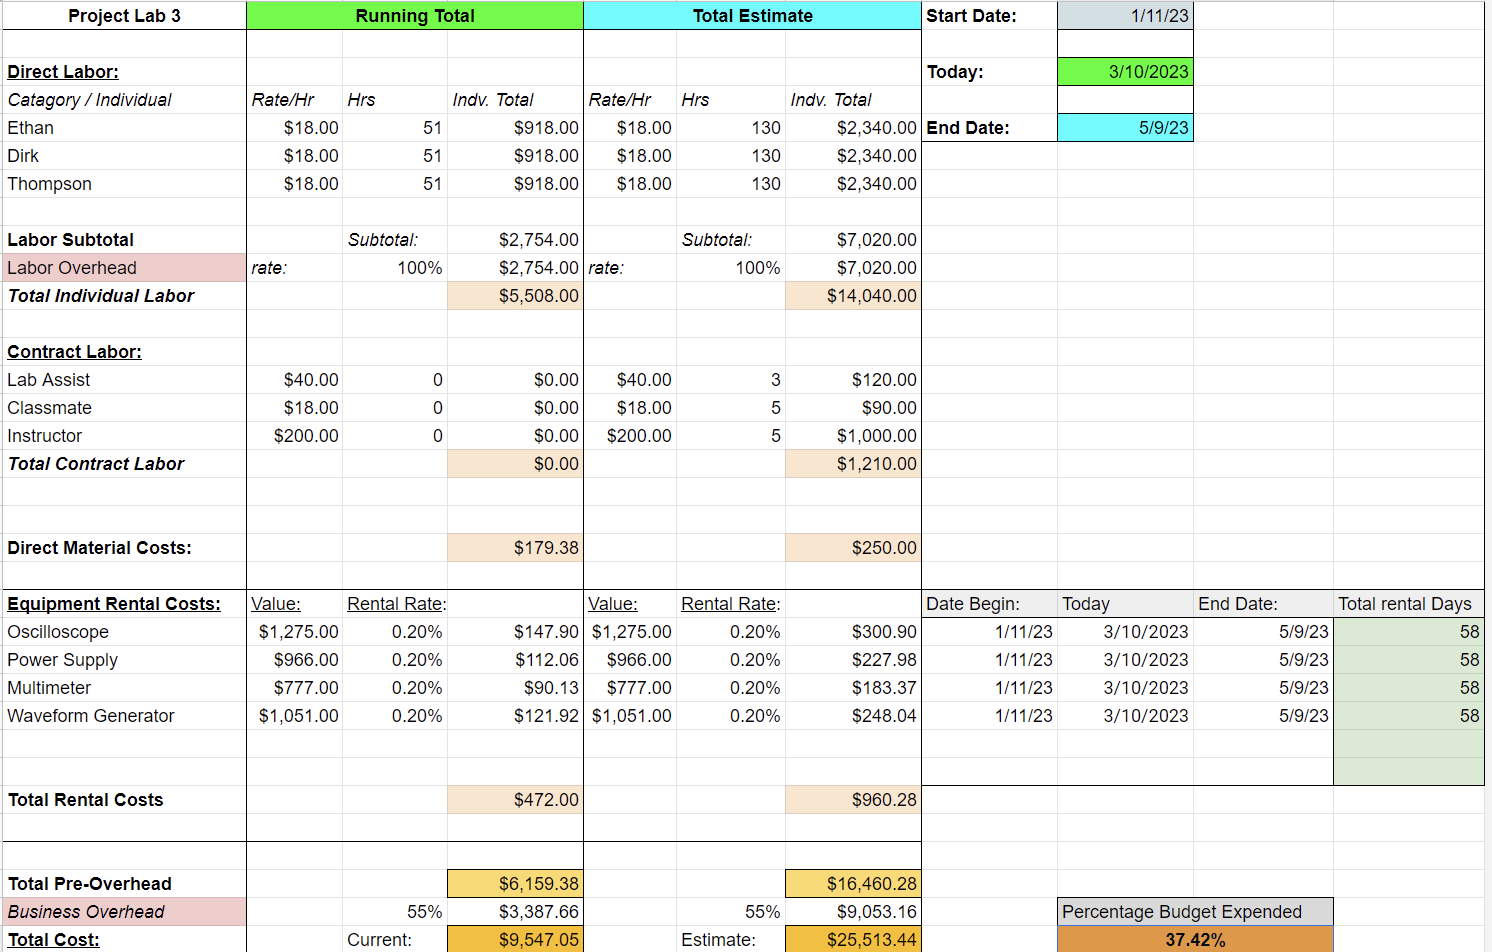
\includegraphics[width=0.75\textwidth]{images/budget.png}
    \caption{Budget}
    \label{budget}
\end{figure}

   As shown in Figure \ref{budget} and \ref{gantt}, the timeline of the project and the budget are currently on task and are much further ahead than expected. The only things left to tackle are debugging and implementatiion of the code onto a test ESP32, then after testing it will be put on to the main ESP32 on the motherboard. 
\subsection{Safety and Ethics}
    Safety-wise, the main issue ot worry about is the security of user's private data, as a user who might be comfortable with their body may not want their heart rate and body temperature to be exposed to the mainstream world after a simple workout. Luckily, Firebase provides built-in security for the variables in each database.
\newpage
\printbibliography

\end{document}